\documentclass{article}
\usepackage{mathtools}
\usepackage{amssymb}
\usepackage{amsthm}
\usepackage{graphicx}
\title{Assignment 3}
\date{Sepetember 15, 2020}
\author{Haixiang Zhu}
\begin{document}
\maketitle
\begin{enumerate}
    \item From the second question of problem set 2, we have
    \begin{equation*}
        \left\{\begin{aligned}
            &c_t=f(k_t)+(1-\delta)k_t-k_{t+1},\text{ for }t=0,1,\dots,T\\
            &{u}'(c_t)=\beta[{f}'(k_{k+1})+(1-\delta)]{u}'(c_{t+1}),\text{ for }t=0,1,\dots,T-1\\
            &k_{T+1}=0
        \end{aligned}\right.
    \end{equation*}
    Setting up the model: $\delta=0.1,\alpha=0.3,\beta=0.96,\sigma=2,k_0 = 0.01$, $f(k)=k^{0.3},$ and $u(c)=1-c^{-1}$.
    \begin{enumerate}
        \item T=1
        \begin{enumerate}
            \item All conditions for solving allocations$\{c_t,k_{t+1}\}_{t=0}^1$:
            \begin{equation*}
                \left\{
                    \begin{aligned}
                    &c_0=0.01^{0.3}+(1-0.1)\times0.01-k_1\\
                    &c_1=k_1^{0.3}+(1-0.1)k_1-k_2\\
                    &c_0^{-2}=0.96\times(1-0.1+0.3k_1^{-0.7})c_1^{-2}\\
                    &k_2=0
                    \end{aligned}
                \right.
            \end{equation*}
            \item Reduced form
            \begin{equation*}
                (0.01^{0.3}+0.009-k_1)^{-2}-0.96(0.9+0.3k_1^{-0.7})(k_1^{0.3}+0.9k_1)^{-2}=0
            \end{equation*}
            Numerical results(See attached Matlab code ``ps3\_1a.m'' and ``fun\_1a.m'')
            \begin{equation*}
                \left\{
                    \begin{aligned}
                    &c_0=0.2200\\
                    &c_1=0.4173\\
                    &k_1=0.0402\\
                    &k_2=0
                    \end{aligned}
                \right.
            \end{equation*}
        \end{enumerate}
        \item T=2
        \begin{enumerate}
            \item All conditions for solving allocations$\{c_t,k_{t+1}\}_{t=0}^2$
            \begin{equation*}
                \left\{
                    \begin{aligned}
                    &c_0=0.01^{0.3}+(1-0.1)\times0.01-k_1\\
                    &c_1=k_1^{0.3}+(1-0.1)k_1-k_2\\
                    &c_2=k_2^{0.3}+(1-0.1)k_2-k_3\\
                    &c_0^{-2}=0.96\times(1-0.1+0.3k_1^{-0.7})c_1^{-2}\\
                    &c_1^{-2}=0.96\times(1-0.1+0.3k_2^{-0.7})c_2^{-2}\\
                    &k_3=0
                    \end{aligned}
                \right.
            \end{equation*}
            \item Reduced form
            \begin{equation*}
                \left\{
                    \begin{aligned}
                        &(0.01^{0.3}+0.009-k_1)^{-2}-0.96(0.9+0.3k_1^{-0.7})(k_1^{0.3}+0.9k_1-k_2)^{-2}=0\\
                        &(k_1^{0.3}+0.9k_1-k_2)^{-2}-0.96(0.9+0.3k_2^{-0.7})(k_2^{0.3}+0.9k_2)^{-2}=0
                    \end{aligned}
            \right.   
            \end{equation*}
            Numerical results(See attached Matlab code ``ps3\_1b.m'' and ``fun\_1b.m'')
            \begin{equation*}
                \left\{
                    \begin{aligned}
                    &c_0=0.2079\\
                    &c_1=0.3682\\
                    &c_2=0.5704\\
                    &k_1=0.0523\\
                    &k_2=0.0915\\
                    &k_3=0
                    \end{aligned}
                \right.
            \end{equation*}
            \item Comparasion between Cass-Koopmans model and Solow model with respect to saving rate
            \begin{equation*}
                \left\{
                    \begin{aligned}
                    &s_0=0.1724\\
                    &s_1=0.1077\\
                    &s_2=-0.1688
                    \end{aligned}
                \right.
            \end{equation*}
            In Cass-Koopmans Model, the savings rate is endogenous and varies from time to time. The savings rate at the period before the last period must be negative.
            As for Solow Model, the steady-state savings rate is exogenous, while the savings rate given by the Golden Rule is endogenous. 
        \end{enumerate}
        \item T=200\\
        All conditions are as follows.
        \begin{gather*}
            \left\{\begin{aligned}
                &\begin{split}
                    [k_t^\alpha+(1-\delta)k_t-k_{t+1}]^{-\sigma}&-\beta[(1-\delta)+\alpha k_{t+1}^{\alpha-1}]\\
                    &\cdot[k_{t+1}^\alpha+(1-\delta)k_{t+1}-k_{t+2}]^{-\sigma}=0,\forall t=0,1,\dots,T-1
                \end{split}\\
                &k_{T+1}=0
                \end{aligned}\right.
        \end{gather*}
        The Matlab code is in attached file ``ps3\_1c.m'' and ``fun\_1c.m''.
        \begin{figure}[h!]
            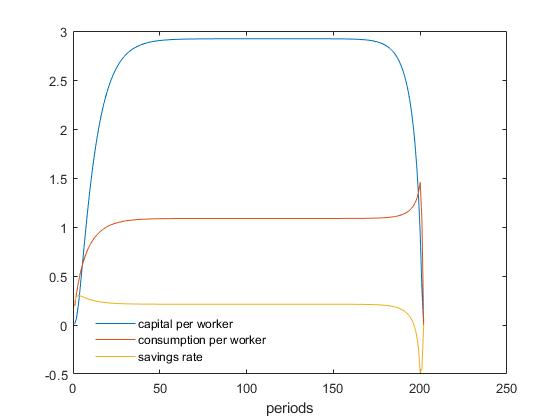
\includegraphics[width=\linewidth]{3_1c.png}
            \caption{The sequences of capital, consumption and savings rate over time}
          \end{figure}
    \end{enumerate}
    \item Full Depreciation
    \begin{enumerate}
        \item Let $t=1-\sigma$. $\sigma\to1\Rightarrow t\to0$\\
        By L'Hopital's rule,
        \begin{equation*}
            \lim_{\sigma\to1}u(c)=\lim_{t\to0}\frac{c^t-1}{t}=\lim_{t\to0}c^t\ln(c)=\ln(c)
        \end{equation*}
        \item Inada conditions
        \begin{proof}
        \begin{align*}
            &f(\cdot):\left\{
                \begin{aligned}
                &\lim_{k\to0}{f}'(k)=\lim_{k\to0}\alpha k^{\alpha-1}=\infty &\alpha\in(0,1)\\
                &\lim_{k\to\infty}{f}'(k)=\lim_{k\to\infty}\alpha k^{\alpha-1}=0 &\alpha\in(0,1)
                \end{aligned}
            \right.\\
            &u(\cdot):\left\{
                \begin{aligned}
                &\lim_{c\to0}{u}'(c)=\lim_{c\to0}c^{-1}=\infty\\
                &\lim_{c\to\infty}{u}'(c)=\lim_{c\to\infty}c^{-1}=0
                \end{aligned}
            \right.
        \end{align*}
        \end{proof}
        \item Euler equation
        \begin{equation*}
            \begin{split}
                {u}'[f(k_t)+(1-\delta)k_t-k_{t+1}]=&\beta[{f}'(k_{t+1})+(1-\delta)]\\
                &\cdot{u}'[f(k_{t+1})+(1-\delta)k_{t+1}-k_{t+2}],\forall t=0,1,\dots,T-1
            \end{split}
        \end{equation*}
        Plugging ${u}(c)=\ln(c),\delta=1,{f}(k)=k^\alpha$, we have
        \begin{align*}
            &\frac{1}{k_t^\alpha-k_{t+1}}=\frac{\alpha\beta k_{t+1}^{\alpha-1}}{k_{t+1}^\alpha-k_{t+2}},\forall t=0,1,\dots,T-1\\
            \Rightarrow&\frac{k_{t+1}^\alpha-k_{t+2}}{k_{t+1}^{\alpha}}=\alpha\beta\frac{k_t^\alpha-k_{t+1}}{k_{t+1}},\forall t=0,1,\dots,T-1
        \end{align*}
        Substituting $z_t=\frac{k_t}{k_{t-1}^\alpha}$, we obtain
        \begin{align*}
            &1-z_{t+2}=\alpha\beta\left(\frac{1}{z_{t+1}}-1\right),\forall t=0,1,\dots,T-1\\
            \Rightarrow&z_{t+1}=1+\alpha\beta-\frac{\alpha\beta}{z_t},\forall t=1,2,\dots,T
        \end{align*}
        \begin{figure}[h!]
            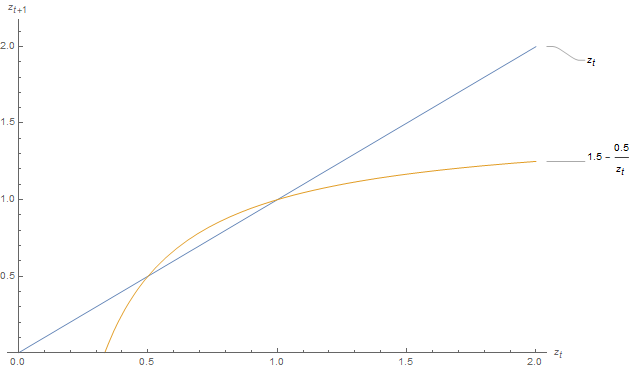
\includegraphics[width=\linewidth]{3_2c.png}
            \caption{$z_{t+1}$ against $z_t$ $(\alpha\beta=0.5)$}
          \end{figure}
        \item 
        \begin{proof}
            \begin{align*}
                \because\,&z_t=\frac{\alpha\beta}{1+\alpha\beta-z_{t+1}},\forall t=1,2,\dots,T\\
                &z_{T+1}=0\\
                \therefore\,&z_T=\frac{\alpha\beta}{1+\alpha\beta}\\
                &z_{T-1}=\alpha\beta\frac{1+\alpha\beta}{1+\alpha\beta+(\alpha\beta)^2}\\
                &z_{T-2}=\alpha\beta\frac{1+\alpha\beta+(\alpha\beta)^2}{1+\alpha\beta+(\alpha\beta)^2+(\alpha\beta)^3}\\
                &\cdots\\
                &z_{T-k}=\alpha\beta\frac{\sum_{i=0}^k(\alpha\beta)^i}{\sum_{i=0}^{k+1}(\alpha\beta)^i}
                =\alpha\beta\frac{1-(\alpha\beta)^{k+1}}{1-(\alpha\beta)^{k+2}},\forall k=0,1,\dots,T-1
            \end{align*}
            Let $t=T-k$, then \(k=T-t\). 
            \begin{equation*}
                z_t=\alpha\beta\frac{1-(\alpha\beta)^{T-t+1}}{1-(\alpha\beta)^{T-t+2}},\forall t=1,2,\dots,T
            \end{equation*}
            And since $z_{T+1}=0$, 
            \begin{equation*}
                z_t=\alpha\beta\frac{1-(\alpha\beta)^{T-t+1}}{1-(\alpha\beta)^{T-t+2}},\forall t=1,2,\dots,T+1
            \end{equation*}
        \end{proof}
        \item Plugging $z_t=\frac{k_t}{k_{t-1}^\alpha}$,
        \begin{equation*}
            \frac{k_t}{k_{t-1}^\alpha}=\alpha\beta\frac{1-(\alpha\beta)^{T-t+1}}{1-(\alpha\beta)^{T-t+2}},\forall t=1,2,\dots,T+1
        \end{equation*}
        Rewriting it as
        \begin{equation*}
            k_{t+1}=\alpha\beta\frac{1-(\alpha\beta)^{T-t}}{1-(\alpha\beta)^{T-t+1}}k_t^\alpha,\forall t=0,1,\dots,T
        \end{equation*}
    \end{enumerate}
\end{enumerate}
\end{document}